\section{Data records}
\label{sec:Data_records}
Digital scans of the original data sheets containing the raw vehicle data are attached in the appendix. Furthermore, it was digitized into a Google-Spreadsheet-Dataset \cite{dataset_google_sheets}, specifically in the sub-spreadsheet "Group 1". The spreadsheet with some evalutations of the data shown in Section \ref{sec:Technical_validation} as well as the Latex files for this paper and scans of the original data sheets are also available on GitHub \cite{github}.

The data set is composed of four different sections for each experiment with each section containing four tables of all measurements. The amount of vehicles for each minute is summed up. Therefore, the seconds are not represented in the Google data set. For instance, if the timestamps for two cars are 0:12 and 0:59, they would both count for the first minute of the experiment in the table. The timestamps are listed in the far left column. 

If cars, buses, motorcycles or trams simultaneously took the same path during the same minute, the sum of all vehicles was noted and the number of buses/motorcycles/trams was specified in brackets. For example, if four cars and a bus took the same path within the same minute, it would be noted as "5 (1 Bus)" in the table. A snippet of a Google table is presented in Figure \ref{fig:google_table_screenshot}, which shows the experiment section, timestamp and direction columns, as well as the latter example.

~\\
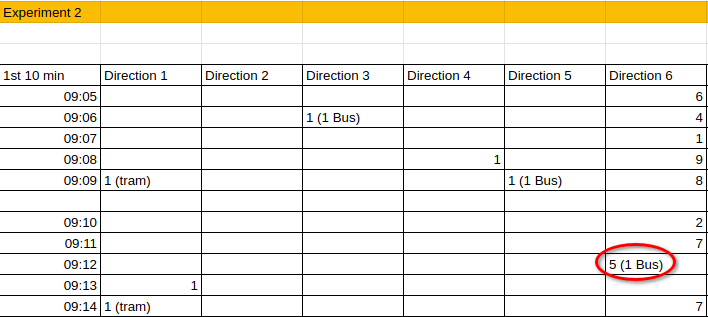
\includegraphics[width=0.95\linewidth]{Screenshot_20220613_112904.png}
\captionof{figure}{Snippet of Google spreadsheet table for Experiment 2}
\label{fig:google_table_screenshot}
